% DO NOT COMPILE THIS FILE DIRECTLY!
% This is included by the other .tex files.

\begin{frame}[t,plain]
\titlepage
\end{frame}

\begin{frame}
    \frametitle{Objectives}
    \begin{itemize}
        \item The 2-day session objective is to show and practice {\bf structured information-exchange} and sharing among team members, SOCs, CSIRT and LEA partners.
        \item The main objective is to be able to map real cases (based on practices from the previous modules) into structured and shareable information.
        \item The session will be interactive and access will be given to a MISP training instance. 
        \item At the end of the 2-day module, you will be able to use MISP and {\bf better undertand sharing practices} among different actors.
    \end{itemize}
    \note[item]{The goal is not to go for full technical session (even if there are some interesting labs) but the focus is the ability to describe cases into structured intelligence to server sharing. Sharing aspect is not only with third parties or partners but it's also within a team or a joint investigation team. This module is also the opportunity to setup and share the access to the MISP training instance which will be used for the 2-day session.} 
\end{frame}

\begin{frame}
\frametitle{MISP - Open Source Threat Intelligence Platform}
        \begin{itemize}
                \item MISP is an open source software (can be self-hosted or cloud-based) {\bf information sharing and exchange platform}
                \item It enables analysts from different sectors/orgs to create, collaborate on and share information
                \item The information shared can then be used to find correlations as well as automatically be fed into {\bf protective tools or processes}
                \item The software is widely used by CERTs, ISACs, Intelligence Community, military organisations, private sector organisations and researchers since 2012
                \item CIRCL is both the main driving force behind the tool's {\bf development} as well as some of the largest information {\bf sharing communities} worldwide
        \end{itemize}
\end{frame}

\begin{frame}
        \frametitle{MISP Project Overview}
        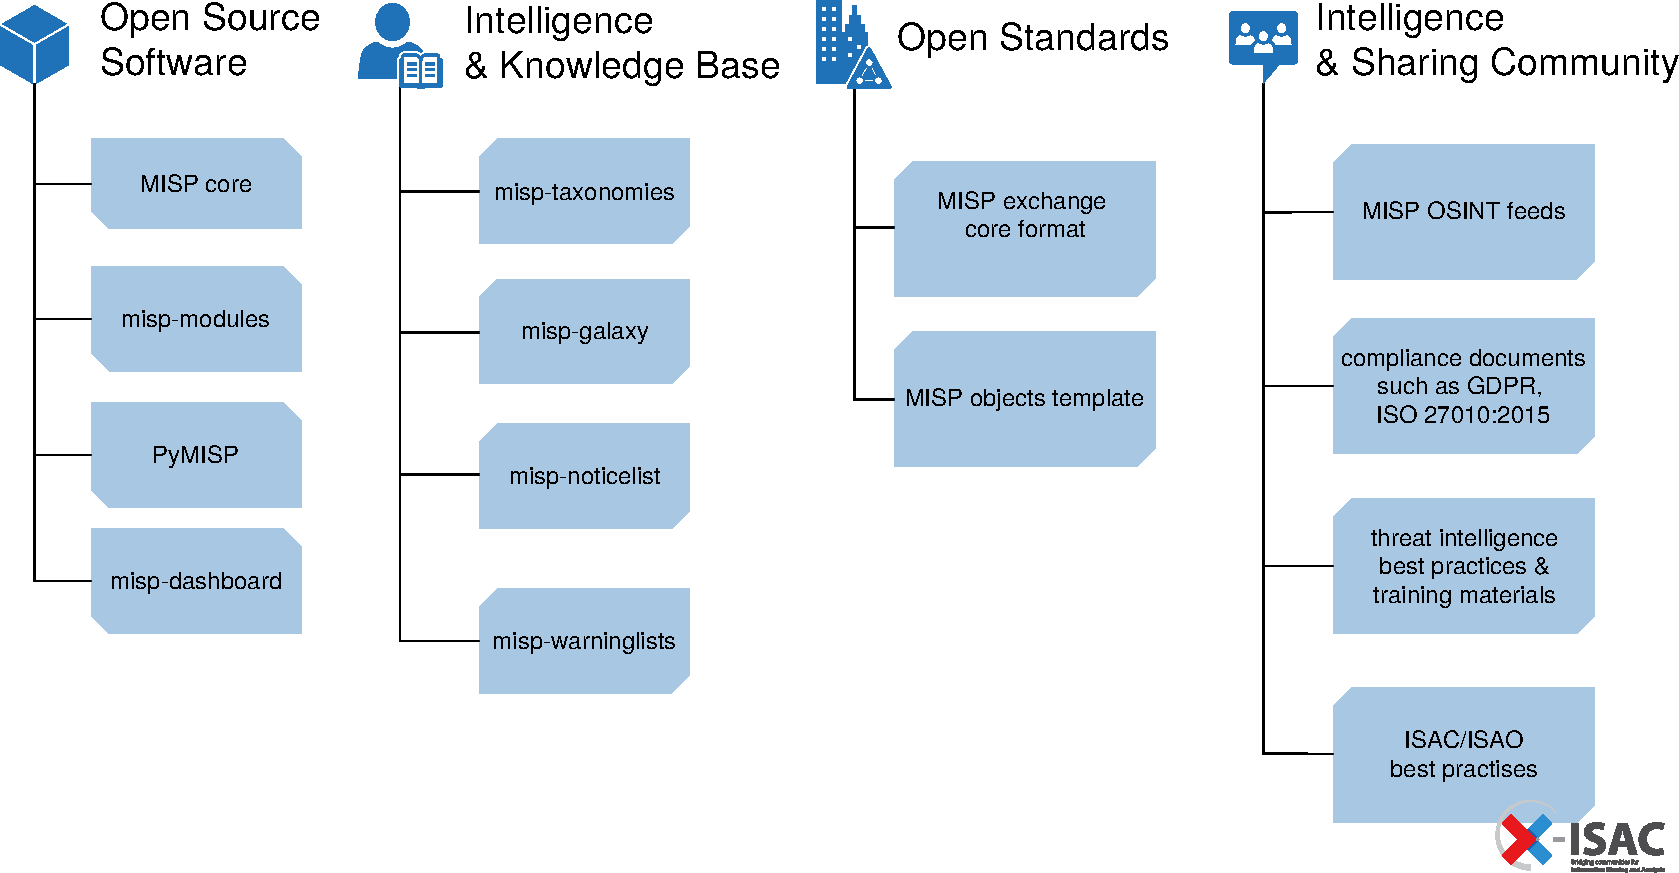
\includegraphics[scale=0.42]{misp-overview-simplified.pdf}\\
    \note[item]{The MISP project includes:}
    \note[item]{Software (the MISP core software itself along with supporting libraries such as PyMISP)}
    \note[item]{Contextualisation libraries (to further elaborate on data's relevance, distribution rules, prevention methods, objectives, etc)}
    \note[item]{Best practice guidance (to ensure cohesion within communities and common understanding of the information shared)}
    \note[item]{Compliance guidance (to go into details about how information sharing fits into the various legal frameworks)}
\end{frame}


\begin{frame}
\frametitle{MISP core distributed sharing functionality}
\begin{itemize}
\item Everyone can be a consumer and/or a contributor/producer.
\item Quick benefit without the obligation to contribute.
\item Low barrier access to get acquainted to the system.
\end{itemize}
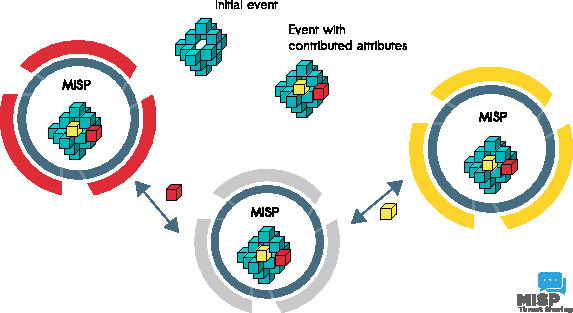
\includegraphics[scale=0.9]{misp-distributed.pdf}
    \note[item]{It is important to emphasise the ability and expectations that come with MISP being a sharing platform rather than a feed ingestion platform}
    \note[item]{Whilst sharing is by no means a requirement in most MISP communities, it is a powerful tool to get sector / region specific information out in the community - especially when it leads to comments, improvements and competitve analyses}
    \note[item]{Having a natural growth in usage patterns is expected, getting started is as easy as logging onto a hosted instance and users can scale out to running their own communities and interconnecting with others organically}
\end{frame}

\begin{frame}
\frametitle{DFIR and MISP digital evidences}
        \begin{itemize}
                \item {\bf Share analysis and report} of digital forensic evidences.
                \item {\bf Propose changes} to existing analysis or report.
                \item Extending existing event with additional evidences for local or limited use (sharing can be defined at event level or attribute level).
                \item {\bf Evaluate correlations}\footnote{MISP has a flexible correlation engine which can correlate on 1-to-1 value but also fuzzy hashing (e.g. ssdeep) or CIDR block matching.} of evidences against external or existing attributes.
                \item {\bf Report sighting} such as false-positive or true-positive (e.g. a partner/analyst has seen a similar indicator).
        \end{itemize}
    \note[item]{Modelling data correctly is essential for finding links to existing data, being able to feed other tools and to have a common understanding of what is meant.}
\end{frame}

\begin{frame}
\frametitle{LEA benefits of using MISP}
\begin{itemize}
        \item  Leverage the long-standing experience in information sharing
        \item  {\bf Bridge their use-cases} with MISP's information sharing mechanisms
        \item {\bf Accessing existing MISP information sharing communities} by getting actionable information from CSIRTs/CERTs networks or security researchers.
        \begin{itemize}
            \item Access to {\bf actionable intelligence} by CSIRT networks
            \item Data-sets can be used to support forensic cases
        \end{itemize}
        \item {\bf Bridging} LE communities with other communities
        \begin{itemize}
            \item Use {\bf sharing groups} to manage distribution across the communities
            \item Safety nets via {\bf synchronisation filters}
            \item Possibility to use certain communities as {\bf correlation sources} only
        \end{itemize}
\end{itemize}
    \note[item]{Explain the advantages of receiving and interacting with the data shared in CSIRT networks}
    \note[item]{Cross correlating data can save time at the initial stages of an investigation}
    \note[item]{For forensics cases, determining if a system was compromised before gather evidences is crucial}
    \note[item]{Sharing can be a vehicle for collaboration, asking for support}
    \note[item]{It is easily possible to only exchange the none sensitive, technical subset of the data when engaging CSIRTs}
\end{frame}

\begin{frame}
\frametitle{LEA benefits of using MISP}
\begin{itemize}
        \item MISP handles a host of additional tasks around the data received and shared by LEAs:
        \begin{itemize}
            \item {\bf Normalisation} to ensure reusability
            \item {\bf Enrichment} using other services
            \item {\bf Correlation} of own cases against community data
            \item Conversion to {\bf other formats}
        \end{itemize}
        \item The {\bf MISP standard format} is extremely flexible
        \begin{itemize}
            \item Create a new {\bf object template} in under 30 minutes
            \item Shared data using custom templates immediately understood by other communities
            \item Tight {\bf validation} and {\bf conversions} for building blocks of the custom templates
        \end{itemize}
\end{itemize}
    \note[item]{Modelling data correctly is essential for finding links to existing data, being able to feed other tools and to have a common understanding of what is meant.}
    \note[item]{Information in general always evolves over time, be it from new findings, other parties observing similar cases or simply by lookup services offering more relevant information over time.}
    \note[item]{New attack techniques often require new ways of modelling information. The time spent waiting for support in tools for new data models is time lost in effectively sharing the information, custom templating is meant to address this.}
\end{frame}

\begin{frame}
        \frametitle{Future of Information Sharing}
        \begin{itemize}
        \item MISP is a long-term project (started in 2012)
        \item{\bf Information sharing is becoming more essential} than ever to thwart threats
        \item Heavy focus on cross-sectorial sharing
        \item Support emerging threats, such as hybrid threats
        \item Open tools and standards along with interoperable software (e.g. DFIR tools) are driving forces behind resilient information exchange communities
        \item Getting ideas and practical {\bf use-cases from LE community} is vital
        \item Reach out to influence how it evolves!
        \end{itemize}
    \note[item]{Something to emphasise here is the emergence of threats spanning multiple disciplines (election interference, fraud involving crypto currencies, etc)}
    \note[item]{Interoperability between organisations and tools if becoming more crucial the more interconnected we are}
    \note[item]{Mention the need for experts to give feedback and input on better modelling strategies, emerging new threats or new classification systems to ensure community cohesion}
\end{frame}


